\documentclass[tikz,border=5pt]{standalone}
\usepackage{tikz}
\usetikzlibrary{shapes.geometric,arrows.meta,positioning}

\begin{document}
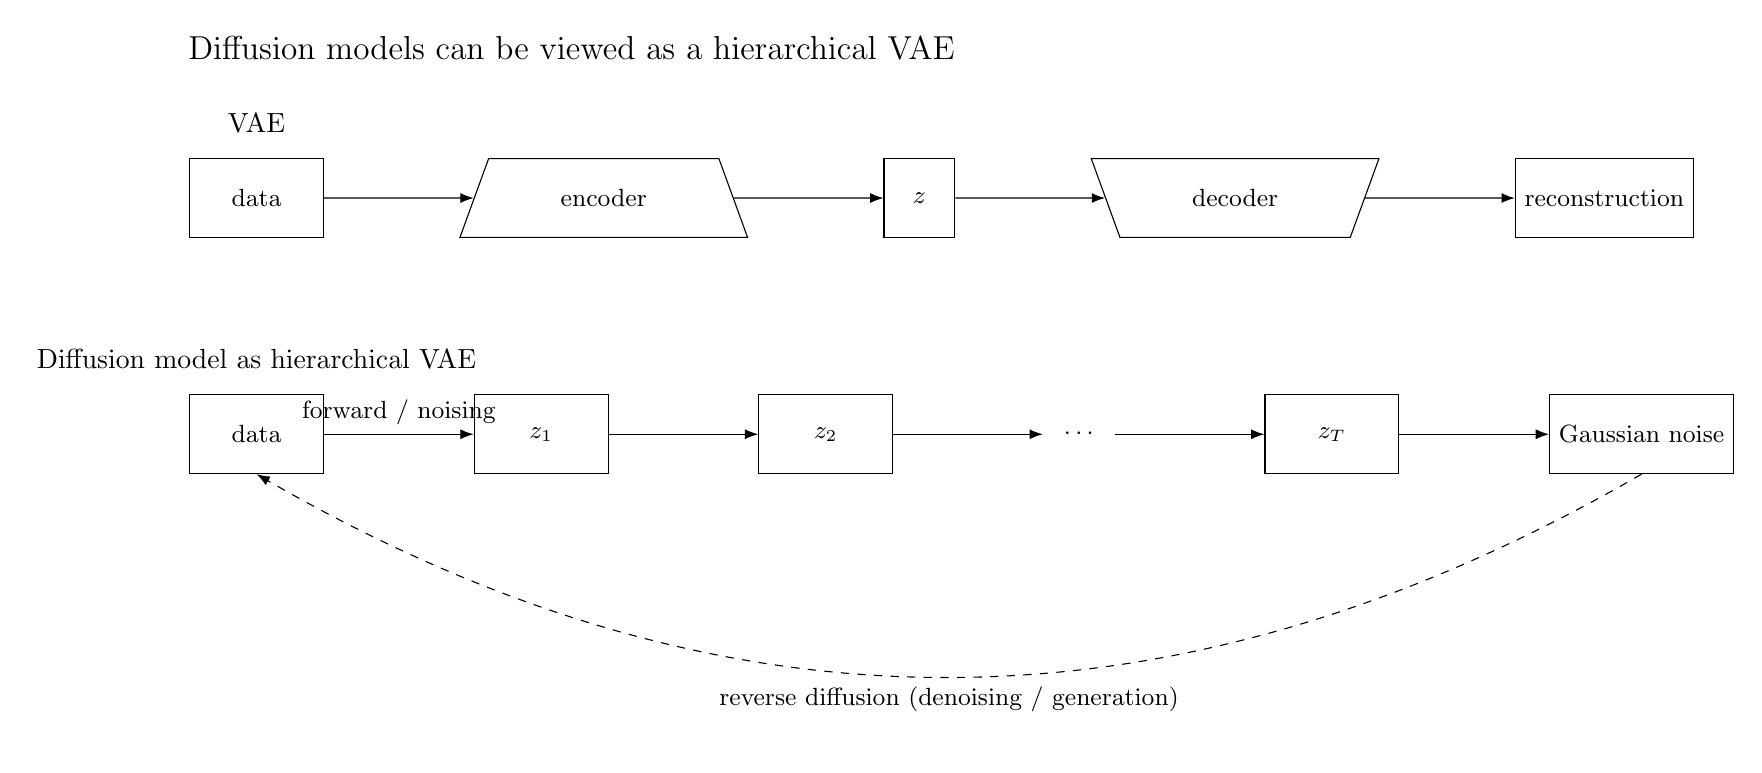
\begin{tikzpicture}[
    >=Latex,
    node distance=1.9cm,
    box/.style={draw, minimum width=1.7cm, minimum height=1cm, align=center},
    tri/.style={draw, trapezium, trapezium angle=70, minimum width=1.4cm, minimum height=1cm, align=center},
    every node/.style={font=\small}
]

% =======================
% Title
% =======================
\node[font=\large, align=center] (title) 
    at (0,3.4) {Diffusion models can be viewed as a hierarchical VAE};

% =======================
% VAE (top row)
% =======================
\node[box] (data) at (-4,1.5) {data};
\node[tri, right=of data] (enc) {encoder};
\node[box, right=of enc, minimum width=0.9cm] (z) {$z$};
\node[tri, right=of z, shape border rotate=180] (dec) {decoder};
\node[box, right=of dec] (out) {reconstruction};

\draw[->] (data) -- (enc);
\draw[->] (enc) -- (z);
\draw[->] (z) -- (dec);
\draw[->] (dec) -- (out);

\node[above=0.2cm of data, font=\normalsize] {VAE};

% =======================
% Diffusion model as hierarchical VAE (bottom row)
% =======================
% forward (noising)
\node[box] (ddata) at (-4,-1.5) {data};
\node[box, right=of ddata] (z1) {$z_1$};
\node[box, right=of z1] (z2) {$z_2$};
\node[box, right=of z2, minimum width=0.9cm, draw=none] (dots) {$\cdots$};
\node[box, right=of dots] (zT) {$z_T$};
\node[box, right=of zT, minimum width=2.2cm] (noise) {Gaussian noise};

\draw[->] (ddata) -- node[above]{forward / noising} (z1);
\draw[->] (z1) -- (z2);
\draw[->] (z2) -- (dots);
\draw[->] (dots) -- (zT);
\draw[->] (zT) -- (noise);

\node[above=0.2cm of ddata, font=\normalsize] 
    {Diffusion model as hierarchical VAE};

% reverse (denoising / generation)
\draw[->, dashed, bend left=30] (noise.south) to node[below]{reverse diffusion (denoising / generation)} (ddata.south);

\end{tikzpicture}
\end{document}
